\documentclass[10pt]{article}
\usepackage[utf8]{inputenc}
\usepackage[T1]{fontenc}
\usepackage{amsmath}
\usepackage{amsfonts}
\usepackage{amssymb}
\usepackage[version=4]{mhchem}
\usepackage{stmaryrd}
\usepackage{graphicx}
\usepackage[export]{adjustbox}
\graphicspath{ {./images/} }
\usepackage{caption}
\usepackage{hyperref}
\hypersetup{colorlinks=true, linkcolor=blue, filecolor=magenta, urlcolor=cyan,}
\urlstyle{same}

\title{A Toolbox for Cryptanalysis: Linear and Affine Equivalence Algorithms* }

\author{Alex Biryukov, Christophe De Cannière ${ }^{\star \star}$, An Braeken**, and Bart Preneel\\
Katholieke Universiteit Leuven, Dept. ESAT/SCD-COSIC, Kasteelpark Arenberg 10, B-3001 Leuven-Heverlee, Belgium\\
\{alex.biryukov, christophe.decanniere, an.braeken, bart.preneel\}@esat.kuleuven.ac.be}
\date{}


%New command to display footnote whose markers will always be hidden
\let\svthefootnote\thefootnote
\newcommand\blfootnotetext[1]{%
  \let\thefootnote\relax\footnote{#1}%
  \addtocounter{footnote}{-1}%
  \let\thefootnote\svthefootnote%
}

%Overriding the \footnotetext command to hide the marker if its value is `0`
\let\svfootnotetext\footnotetext
\renewcommand\footnotetext[2][?]{%
  \if\relax#1\relax%
    \ifnum\value{footnote}=0\blfootnotetext{#2}\else\svfootnotetext{#2}\fi%
  \else%
    \if?#1\ifnum\value{footnote}=0\blfootnotetext{#2}\else\svfootnotetext{#2}\fi%
    \else\svfootnotetext[#1]{#2}\fi%
  \fi
}

\begin{document}
\maketitle
\captionsetup{singlelinecheck=false}


\begin{abstract}
This paper presents two algorithms for solving the linear and the affine equivalence problem for arbitrary permutations (S-boxes). For a pair of $n \times n$-bit permutations the complexity of the linear equivalence algorithm (LE) is $O\left(n^{3} 2^{n}\right)$. The affine equivalence algorithm (AE) has complexity $O\left(n^{3} 2^{2 n}\right)$. The algorithms are efficient and allow to study linear and affine equivalences for bijective S -boxes of all popular sizes (LE is efficient up to $n \leq 32$ ). Using these tools new equivalent representations are found for a variety of ciphers: Rijndael, DES, Camellia, Serpent, Misty, Kasumi, Khazad, etc. The algorithms are furthermore extended for the case of non-bijective $n$ to $m$-bit S-boxes with a small value of $|n-m|$ and for the case of almost equivalent S-boxes. The algorithms also provide new attacks on a generalized Even-Mansour scheme. Finally, the paper defines a new problem of S-box decomposition in terms of Substitution Permutations Networks (SPN) with layers of smaller S-boxes. Simple information-theoretic bounds are proved for such decompositions.
\end{abstract}

Keywords: Linear, affine equivalence algorithm, S-boxes, Block-ciphers, Rijndael, DES, Cryptanalysis, Algebraic attacks, S-box decomposition, Side-channel attacks.

\section*{1 Introduction}
In this paper we study invariant properties of permutations ( S -boxes) under the action of groups of linear or affine mappings. By using a cryptanalytic approach to this problem we provide efficient algorithms for detecting linear and affine equivalences. Linear/affine equivalence problems are of interest in various areas of mathematics. It is also a natural problem for a cryptanalyst/cipher designer

\footnotetext{\begin{itemize}
  \item The work described in this paper has been supported in part by the Commission of the European Communities through the IST Programme under Contract IST-199912324 and by the Concerted Research Action (GOA) Mefisto.\\
${ }^{\star \star}$ F.W.O. Research Assistant, sponsored by the Fund for Scientific Research - Flanders (Belgium).
\end{itemize}
}
to look at, since basic properties of S-boxes, such as differential [7] and linear properties 20 are invariant under these transformations. An efficient algorithmic tool allows to study the properties of a whole equivalence class by analyzing a single representative. Further motivations to study this problem are: deeper understanding of Rijndael (AES) [13] - a block cipher with nice algebraic structure; recent interest in potential algebraic attacks 1022 ; and the discovery of a variety of equivalent representations for the AES 415 and other ciphers. Such representations help to describe ciphers with simpler systems of low-degree equations, allow more efficient implementations, and are very useful in the design of countermeasures against side-channel attacks. These problems show that it is essential to have a toolbox of generic algebraic algorithms for the analysis and design of block ciphers. This paper makes one step in this direction.

We provide algorithms that can quickly test if two S -boxes $S_{1}$ and $S_{2}$ are equivalent, i.e., if there exist (linear or affine) mappings $A_{1}, A_{2}$ such that $A_{2} \circ S_{1} \circ A_{1}=S_{2}$. The complexity of our linear equivalence algorithm (LE) is $O\left(n^{3} 2^{n}\right)$, and the affine equivalence algorithm (AE) has complexity $O\left(n^{3} 2^{2 n}\right)$. Within these complexities, both algorithms will either return the mappings $A_{1}$ and $A_{2}$, or detect that the S -boxes are inequivalent. This should be compared with $O\left(2^{n^{2}}\right)$ for a naive algorithm that guesses one of the mappings. We solve the affine equivalence problem by finding unique representatives for the linear equivalence classes - a method of interest in itself. The efficiency of the given algorithms allows to find linear equivalences for $n$ up to 32 and affine equivalences for $n$ up to 17 , which covers most of the S -boxes used in modern symmetric primitives and allows to study partial functions composed of several S-boxes and portions of the mixing layers. We extend our results for the case of non-bijective S-boxes with $n$ input bits and $m$ output bits when the input/output deficiency $|n-m|$ is small. Another interesting extension is the search for almost equivalent S boxes, which is as efficient as the basic algorithms. This tool will be of interest to the cryptanalyst/cipher designer since it allows to check quickly if a certain S-box is close to the set of affine functions or if two S-boxes, one with unknown structure and the other with known algebraic structure are almost equivalent. This approach induces an interesting metric in the space of affine equivalence classes of S-boxes.

Using our toolbox of algorithms we find that many S-boxes of popular ciphers are self-affine equivalent, which allows to produce equivalent representations of these ciphers. Among the examples are: AES (for which we show more non-trivial dual ciphers than in "The Book of Rijndaels" 4]), DES, Serpent, Misty, Kasumi, Khazad, etc. We also compare the original S-boxes of DES and the strengthened set $S^{5} \mathrm{DES}$ [18]. It is easy to observe that there is much less variety in the set of classes of the more recent S -boxes, which is a consequence of the introduction of additional design criteria.

We also show that our algorithms can be viewed as attack algorithms against a generalized Even-Mansour scheme (with secret affine mappings instead of XORs of constant secret keys). Finally we introduce a new S-box decomposition problem: the problem of finding SPNs with layers of smaller S-boxes equivalent\\
to a single large S-box. This problem is natural in the context of algebraic attacks on ciphers and also in the context of efficient hardware implementations for large lookup tables. We show simple lower bounds for this S-box decomposition problem. For 8 -bit S-boxes the bound is 20 layers of 4 -bit S-box SPNs, which may imply that 8 -bit S -boxes are too small to withstand potential algebraic attacks 10. Exactly how relevant the algebraic attacks are and whether suboptimal S-box decomposition algorithms exist is a matter of future research.

This paper is organized as follows: in Sect. 2 and 3 we describe our linear equivalence and affine equivalence algorithms. In Sect. 4 we describe extensions of these algorithms to non-bijective S-boxes and to almost-equivalent S-boxes. In Sect. 5 we discuss self-equivalences found in S-boxes of various ciphers and corresponding equivalent representations of AES, DES, Camellia, Serpent, Misty, Kasumi and Khazad. In Sect. 6 we apply our algorithms to a generalized EvenMansour scheme. Sect. 7 provides a few results on the S-box decomposition problem. Finally Sect. 8 summarizes the paper.

\section*{2 The Linear Equivalence Algorithm (LE)}
In this section we provide an efficient algorithm for solving the linear equivalence problem for $n \times n$-bit S-boxes. Here and in the rest of this paper, by linear mapping we mean a mapping $L(x)$ over $G F(2)^{n}$ that satisfies $L(x+y)=L(x)+ L(y)$. It will be useful to think of $L$ as an $n \times n$ matrix. A mapping is called affine if it can be written as $A(x)=L(x)+c$ with some constant $c \in G F(2)^{n}$. The algorithms we will describe can be generalized to arbitrary fields. Note that the algorithm in this section is very similar to the "to and fro" algorithm used to solve the polynomial isomorphism problem for systems of quadratic equations in [23]. This fact was pointed out to us by an anonymous referee.

Let us consider the problem of checking linear equivalence between two permutations (S-boxes) $S_{1}$ and $S_{2}$. The problem is to find two invertible linear mappings $L_{1}$ and $L_{2}$, such that $L_{2} \circ S_{1} \circ L_{1}=S_{2}$. A naive approach would be to guess one of the mappings, for example $L_{1}$. Then one can extract $L_{2}$ from the equation: $L_{2}=S_{2} \circ L_{1}^{-1} \circ S_{1}^{-1}$, and check if it is a linear, invertible mapping. There are $O\left(2^{n^{2}}\right)$ choices of invertible linear mappings over $n$-bit vectors. For each guess one will need about $n^{3}$ steps to check for linearity and invertibility using Gaussian elimination. For large $n$ we could benefit from the asymptotically faster Coppersmith-Winograd's method 11 of $O\left(n^{2.376}\right)$. However, for $n \leq 32$, which is of main practical interest, we can use 32-bit processor instructions to bring the complexity to $n^{2}$ steps. In total the naive algorithm would require $O\left(n^{3} 2^{n^{2}}\right)$ steps (a similar naive affine equivalence algorithm will use $\left.O\left(n^{3} 2^{n(n+1)}\right)\right)$. For $n=6$ this approach will require about $2^{44}$ steps.

Improving the naive approach is easy: we need only $n$ equations in order to check $L_{2}$ for invertibility and linearity. If one guesses only $\log _{2} n$ vectors from $L_{1}$ one may span a space of $n$ points (by trying all linear combinations of the guessed vectors), evaluate the results through $L_{1}, S_{1}$ and $S_{2}$ and have $n$ constraints required to check for linearity of $L_{2}$. If the $n$ new equations are not\\
independent one will need to guess additional vectors of $L_{1}$. Such an algorithm would require guessing of $n \log _{2} n$ bits of $L_{1}$ and the total complexity would be $O\left(n^{3} 2^{n \log n}\right)$. Below we will show a much more efficient algorithm, which stays feasible for much higher values of $n$ (up to $n=32$ ).

Another natural approach to the linear equivalence problem would be to follow a reduction from a Boolean linear equivalence problem. Recently a new heuristic algorithm for the Boolean equivalence problem was described by Fuller and Millan in [15]. They propose an algorithm based on the distribution of the Walsh-Hadamard transform and the autocorrelation. The complexity of this algorithm is roughly $n^{n}$, which is already a higher complexity than for the algorithms we present in this paper. Trying to adapt Fuller-Millan's approach, one might decide to build difference distribution [7] (or linear approximation [20]) tables for the two S -boxes and to match the frequencies between the tables after applying small changes to the S -boxes. However, the construction of a difference distribution table for a $n \times n$-bit S-box requires $O\left(2^{2 n}\right)$ steps and memory; creating a linear approximation table takes $O\left(n 2^{2 n}\right)$ steps and $O\left(2^{2 n}\right)$ memory. Thus an algorithm using frequencies in such tables seems to be lower bounded by $O\left(2^{2 n}\right)$ steps. Note that for strong ciphers frequency profiles in such tables are artificially flattened, which will make any such algorithm even harder to apply.

\subsection*{2.1 Our Linear Equivalence Algorithm}
In our algorithm we exploit two ideas. The first one we call a needlework effect in which guesses of portions from $L_{1}$ provide us with free knowledge of the values of $L_{2}$. These new values from $L_{2}$ allow us to extract new free information about $L_{1}$, etc. This process is supported by a second observation, which we call exponential amplification of guesses, which happens due to the linear (affine) structure of the mappings. The idea is that knowing $k$ vectors from the mapping $L_{1}$, we know $2^{k}$ linear combinations of these vectors for free. Now we are ready to describe our algorithm.

In the description we use the following notation: the linear mappings $L_{1}$ and $L_{2}$ will be denoted by $A$ and $B^{-1}$ respectively. The sets $C_{A}, C_{B}$ are the sets of checked points for which the mapping ( $A$ or $B$ respectively) is known. By construction, these sets will also contain all the linear combinations of known points. The sets $U_{A}, U_{B}$ are the sets of yet unknown points. The sets $N_{A}, N_{B}$ describe all the new points for which we know the mapping (either $A$ or $B$, respectively), but which are linearly independent from points of $C_{A}$ or $C_{B}$, respectively. The sets $C, N$ and $U$ are always disjoint. We introduce the following natural notation for operations on sets:


\begin{align*}
& F(W)=\{F(x) \mid x \in W\}  \tag{1}\\
& W \oplus c=\{x \oplus c \mid x \in W\} . \tag{2}
\end{align*}


Starting with the empty sets $C_{A}, C_{B}$ (no points known), and the complete unknown sets $U_{A}, U_{B}$, we make initial guesses for the value $A(x)$ for some point $x$, and place it into $N_{A}$. Usually two guesses would be sufficient in order to start\\
the exponential amplification process. However we can do better if $S_{1}(0) \neq 0$ and thus $S_{2}(0) \neq \mathrm{d}^{1}$. In such a case we can add the value of 0 to both $N_{A}$ and $N_{B}$. Using the fact that $A(0)=B(0)=0$ we can start with less initial guessing, which saves us a factor of $2^{n}$ in complexity. The algorithm follows the implications of the initial guess until we have enough vectors for $A$ or $B$ to either reach a contradiction or have $n$ independent vectors completely defining the mapping. If we obtain a mapping that is either non-invertible or non-linear, we reject the incorrect guess. Otherwise we check all the points of both mappings to avoid degenerate cases of "almost" affine mappings (we exploit this feature in Sect. 4.3).

Linear Equivalence (LE)

\begin{verbatim}
$U_{A} \Leftarrow\{0,1\}^{n} ; U_{B} \Leftarrow\{0,1\}^{n}$
$N_{A} \Leftarrow \varnothing ; N_{B} \Leftarrow \varnothing$
$C_{A} \Leftarrow \varnothing ; C_{B} \Leftarrow \varnothing$
while ( $U_{A} \neq \varnothing$ and $U_{B} \neq \varnothing$ ) or (All guesses rejected) do
    if $N_{A}=\varnothing$ and $N_{B}=\varnothing$ then
        If previous guess rejected, restore $C_{A}, C_{B}, U_{A}, U_{B}$.
        Guess $A(x)$ for some $x \in U_{A}$
        Set $N_{A} \Leftarrow\{x\}, U_{A} \Leftarrow U_{A} \backslash\{x\}$
    end if
    while $N_{A} \neq \varnothing$ do
        Pick $x \in N_{A} ; N_{A} \Leftarrow N_{A} \backslash\{x\} ; N_{B} \Leftarrow S_{2}\left(x \oplus C_{A}\right) \backslash C_{B}$
        $C_{A} \Leftarrow C_{A} \cup\left(x \oplus C_{A}\right)$
        if $\left|N_{B}\right|+\log _{2}\left|C_{B}\right|>$ const $n$ then
            if $B$ is invertible linear mapping then
                Derive $A$ and check $A, B$ at all points, that are still left in $U_{A}$ and $U_{B}$.
            else
                Reject latest guess; $N_{A} \Leftarrow \varnothing ; N_{B} \Leftarrow \varnothing$
            end if
        end if
    end while
    while $N_{B} \neq \varnothing$ do
        Pick $y \in N_{B} ; N_{B} \Leftarrow N_{B} \backslash\{y\} ; N_{A} \Leftarrow S_{2}{ }^{-1}\left(y \oplus C_{B}\right) \backslash C_{A}$
        $C_{B} \Leftarrow C_{B} \cup\left(y \oplus C_{B}\right)$
        if $\left|N_{B}\right|+\log _{2}\left|C_{B}\right|>$ const $\cdot n$ then
            if $A$ is invertible linear mapping then
                Derive $B$ and check $A, B$ at all points, that are still left in $U_{A}$ and $U_{B}$.
            else
                Reject latest guess; $N_{A} \Leftarrow \varnothing ; N_{B} \Leftarrow \varnothing$
            end if
        end if
    end while
    $U_{A} \Leftarrow U_{A} \backslash C_{A} ; U_{B} \Leftarrow U_{B} \backslash C_{B}$
end while
\end{verbatim}

\footnotetext{${ }^{1}$ If one S-box maps zero to zero and the other does not, they cannot be linearly equivalent.
}\begin{figure}[h]
\begin{center}
  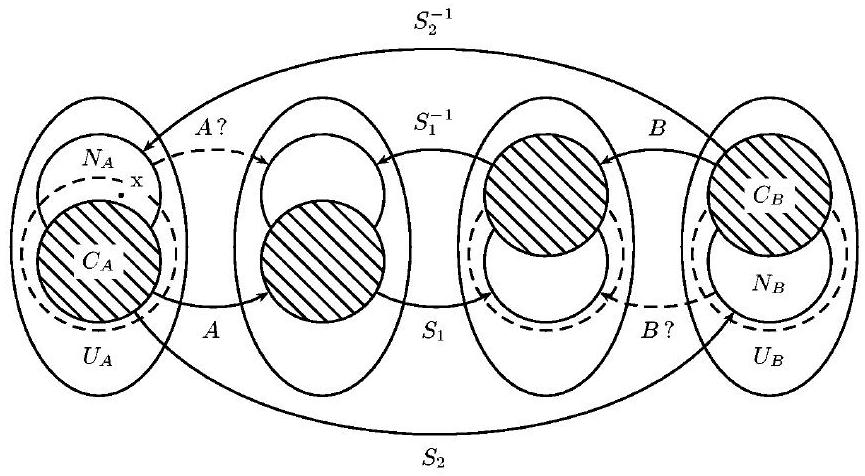
\includegraphics[alt={},max width=\textwidth]{84a1f539-cadb-4d9e-a241-76b2bf1f79cf-06_476_865_149_315}
\captionsetup{labelformat=empty}
\caption{Fig. 1. The relations between the different sets for the LE algorithm.}
\end{center}
\end{figure}

The complexity of this approach is about $n^{3} \cdot 2^{n}$ steps (for S -boxes that do not map zero to zero, and $n^{3} \cdot 2^{2 n}$ otherwise). In practice our algorithms are faster by taking into account 32 -bit operations, which reduce the complexity to $O\left(n^{2} 2^{n}\right)$ as long as $n \leq 32$. For 8 -bit S -boxes it is about $2^{14}$ steps. For 16-bit S-boxes it is $2^{24}$ steps. Table 2 in Appendix A lists the complexities for $n \leq 32$.

\section*{3 The Affine Equivalence Algorithm (AE)}
In this section we generalize the equivalence problem to the affine case. This time we want an algorithm that takes two $n \times n$-bit S-boxes $S_{1}$ and $S_{2}$ as input, and checks whether there exists a pair of invertible affine mappings $A_{1}$ and $A_{2}$ such that $A_{2} \circ S_{1} \circ A_{1}=S_{2}$. Each of these affine mappings can be expressed as a linear transform followed by an addition, which allows us to rewrite the affine equivalence relation as $B^{-1} S_{1}(A \cdot x \oplus a) \oplus b=S_{2}(x), \forall x \in\{0,1\}^{n}$ with $A$ and $B$ invertible $n \times n$-bit linear mappings and with $n$-bit constants $a$ and $b$.

\subsection*{3.1 Basic Algorithm}
As the problem is very similar to the linear equivalence problem, it seems natural to try to reuse the linear algorithm described above. A straightforward solution would be:

\begin{verbatim}
for all a do
    for all b do
        check whether St(x\oplusa) and St{ St) \(x) dinearly equivalent
    end for
end for
\end{verbatim}

This approach adds a factor $2^{2 n}$ to the complexity of the linear algorithm, bringing the total to $O\left(n^{3} 2^{3 n}\right)$. This algorithm is rather inefficient as the linear equivalence needs to be checked for each pair $(a, b)^{2}$ In a second approach, we try

\footnotetext{${ }^{2}$ Another solution is to avoid guessing the constants by considering linear combinations consisting of only an odd number of points. We need three guesses to initiate this process, hence the total complexity is the same.
}
to avoid this by assigning a unique representative to each linear equivalence class. Indeed, if we find an efficient method to identify this representative for a given permutation, then we can check for affine equivalence using the following algorithm:

\begin{verbatim}
for all a do
    insert the representative of the lin. equiv. class of St(x\oplusa) in a table T1
end for
for all b do
    insert the representative of the lin. equiv. class of Se(x)\oplusb in a table T2
end for
if T \ CH2\not= then
    conclude that S and S are affine equivalent
end if
\end{verbatim}

The complexity of this second algorithm is about $2^{n}$ times the work needed for finding the linear representative. If the latter requires less than $O\left(n^{3} 2^{2 n}\right)$, then the second approach will outperform the first. Next, we present an algorithm that constructs the representative in $O\left(n^{3} 2^{n}\right)$. As a result, the total complexity of finding affine equivalences is brought down to $O\left(n^{3} 2^{2 n}\right)$. Table 2 shows these complexities for values of $n \leq 32$. The same complexity estimation holds for the case of inequivalent S-boxes.

An additional interesting property of this approach is that it can efficiently solve the problem of finding mutual equivalences in a large set of S-boxes. Due to the fact that the main part of the computation is performed separately for each S-box, the complexity will grow only linearly with the number of S-boxes (and not with the number of possible pairs).

\subsection*{3.2 Finding the Linear Representative}
The efficiency of an algorithm that finds the linear representative $R_{S}$ for an S-box $S$ depends on how this unique representative is chosen. In this paper, we decide to define it as follows: if all S -boxes in a linear equivalence class are ordered lexicographically according to their lookup tables, then the smallest is called the representative of the class. With this order the smallest permutation is the identity, and for example, permutation $[0,1,3,4,7,2,6,5]$ is smaller than the permutation $[0,2,1,6,7,4,3,5]$.

In order to construct the representative $R_{S}$ for the linear class containing a given S-box $S$, we use an algorithm that is based on the same principles as the algorithm in Sect. 2.1. after making an initial guess, we incrementally build the linear mappings $A$ and $B$ such that $R_{S}^{\prime}=B^{-1} \circ S \circ A$ is as small as possible. This is repeated and the representative $R_{S}$ is obtained by taking the smallest $R_{S}^{\prime}$ over all possible guesses. When explaining the algorithm, we will refer to the same sets $C_{A}, C_{B}, N_{A}, N_{B}, U_{A}$ and $U_{B}$ as in Sect. 2.1 but as their function throughout the algorithm is slightly different, we first reformulate their definition:

\begin{figure}[h]
\begin{center}
  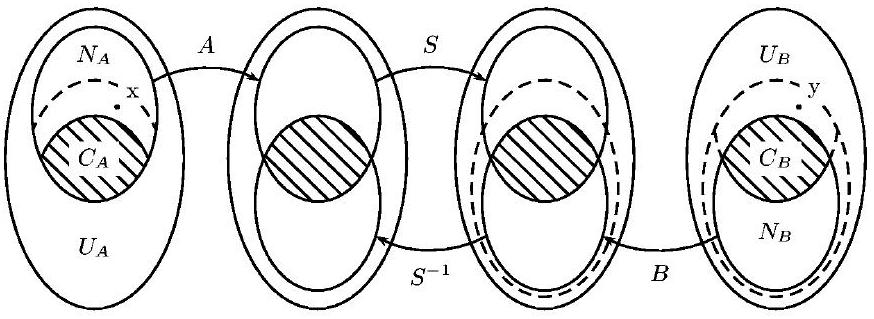
\includegraphics[alt={},max width=\textwidth]{84a1f539-cadb-4d9e-a241-76b2bf1f79cf-08_319_874_156_317}
\captionsetup{labelformat=empty}
\caption{Fig. 2. The relations between the different sets for the AE algorithm.}
\end{center}
\end{figure}

Sets $D_{A}$ and $D_{B}$ - values for which $A$ or $B$ are known respectively. As $A$ is a linear mapping, any linear combination of points of $D_{A}$ will also reside in $D_{A}$. The same is true for $D_{B}$. Note that $D_{A}$ and $D_{B}$ always include 0 .\\
Sets $C_{A}$ and $C_{B}$ - points of $D_{A}$ that have a corresponding point in $D_{B}$ and vice versa, i.e., $S \circ A\left(C_{A}\right)=B\left(C_{B}\right)$. For these values, $R_{S}^{\prime}$ and $R_{S}^{\prime}{ }^{-1}$ are known respectively.\\
Sets $N_{A}$ and $N_{B}$ - remaining points of $D_{A}$ and $D_{B}$. We have that $S \circ A\left(N_{A}\right) \cap B\left(N_{B}\right)=\varnothing$.\\
Sets $U_{A}$ and $U_{B}$ - values for which $A$ and $B$ can still be chosen. It is important to note that the algorithm will update sets $D_{A}$ and $U_{A}$ in such a way that $d<u$ for any $d \in D_{A}$ and $u \in U_{A}$.

The main part of the algorithm that finds a candidate $R_{S}^{\prime}$ consists in repeatedly picking the smallest input $x$ for which $R_{S}^{\prime}$ is not known and trying to assign it to the smallest available output $y$. Using the definitions above, this may be written as:

\begin{verbatim}
while $N_{A} \neq \varnothing$ do
    pick $x=\min _{t \in N_{A}}(t)$ and $y=\min _{t \in U_{B}}(t)$
    complete $B$ such that $B(y)=S \circ A(x)$ and thus $R_{S}^{\prime}(x)=y$
    update all sets according to their definitions
    while $N_{A}=\varnothing$ and $N_{B} \neq \varnothing$ do
        pick $x=\min _{t \in U_{A}}(t)$ and $y=\min _{t \in N_{B}}(t)$
        complete $A$ such that $A(x)=S^{-1} \circ B(y)$ and thus $R_{S}^{\prime}(x)=y$
        update all sets according to their definitions
    end while
end while
\end{verbatim}

When this algorithm finishes, $N_{A}$ and $N_{B}$ are both empty. If $U_{A}$ and $U_{B}$ turn out to be empty as well, then $R_{S}^{\prime}$ is completely defined. In the opposite case, we need to guess $A$ for the smallest point in $U_{A}$. This will add new elements to $N_{A}$, such that we can apply the algorithm once again. To be sure to find the smallest representative, we must repeat this for each possible guess.

In most cases, we will only need to guess $A$ for a single point, which means that about $2^{n}$ possibilities have to be checked. Completely defining $R_{S}^{\prime}$ for a particular guess takes about $2^{n}$ steps. However, most guesses will already be\\
rejected after having determined only slightly more than $n$ values, because at that point $R_{S}^{\prime}$ will usually turn out to be larger than the current smallest candidate. Due to this, the total complexity of finding the representative is expected to be $O\left(n^{3} 2^{n}\right)$.

We now explain how the sets are updated in the previous algorithm. We only consider the case where $N_{A} \neq \varnothing$ and $x=\min _{t \in N_{A}}(t)$, but the other case is very similar. The first step is to use the value of $B(y)$ to derive $B$ for all linear combinations of $y$ and $D_{B}$. This implies that:


\begin{align*}
D_{B}^{\prime} & \Leftarrow D_{B} \cup\left(D_{B} \oplus y\right)  \tag{3}\\
U_{B}^{\prime} & \Leftarrow U_{B} \backslash\left(D_{B} \oplus y\right) . \tag{4}
\end{align*}


Next, the algorithm checks whether any new point inserted in $D_{B}$ has a corresponding point in $D_{A}$ and updates $C_{B}, N_{B}, C_{A}$ and $N_{A}$ accordingly:


\begin{align*}
& C_{B}^{\prime} \Leftarrow C_{B} \cup B^{-1}\left[B\left(D_{B} \oplus y\right) \cap S \circ A\left(N_{A}\right)\right],  \tag{5}\\
& N_{B}^{\prime} \Leftarrow N_{B} \cup B^{-1}\left[B\left(D_{B} \oplus y\right) \backslash S \circ A\left(N_{A}\right)\right],  \tag{6}\\
& C_{A}^{\prime} \Leftarrow C_{A} \cup A^{-1} \circ S^{-1}\left[B\left(D_{B} \oplus y\right) \cap S \circ A\left(N_{A}\right)\right],  \tag{7}\\
& N_{A}^{\prime} \Leftarrow N_{A} \backslash A^{-1} \circ S^{-1}\left[B\left(D_{B} \oplus y\right) \cap S \circ A\left(N_{A}\right)\right] . \tag{8}
\end{align*}


The resulting sets are depicted in dashed lines in Fig. 2

\subsection*{3.3 A Different Approach Using the Birthday Paradox}
The efficiency gain obtained in the previous subsections is due to the fact that the computation is split into two parts, each of which depends on a single S-box $S_{1}$ or $S_{2}$ only. In this subsection, we apply the same idea in a different way and present a second algorithm which is directly based on the birthday method from 23 .

In order to explain the algorithm, we will denote the input and corresponding output values of $S_{1}$ by $x_{1}^{i}$ and $y_{1}^{i}$, with $y_{1}^{i}=S_{1}\left(x_{1}^{i}\right)$. For the second S -box $S_{2}$, we use the notations $x_{2}^{i}$ and $y_{2}^{i}$. Suppose now that we are given a set of pairs $\left(x_{1}^{i}, y_{1}^{i}\right)$ and a second set of pairs $\left(x_{2}^{i}, y_{2}^{i}\right)$, and are asked to determine whether both ordered sets are related by affine transforms, i.e., $x_{1}^{i}=A_{1}\left(x_{2}^{i}\right)$ and $y_{1}^{i}=A_{2}^{-1}\left(y_{2}^{i}\right)$ for all $i$. A straightforward method would be to collect $n+1$ independent equations $x_{1}^{i}=A_{1}\left(x_{2}^{i}\right)$, perform a Gaussian elimination in order to recover the coefficients of $A_{1}$, and verify if this transform holds for the other values in the sets. If it does, this procedure can be repeated for $A_{2}$.

We can as well take a different approach, however. The main observation now is that any linear relation between different $x_{1}^{i}$, containing an even number of terms, must hold for the corresponding values $x_{2}^{i}$ as well, given that $x_{1}^{i}=A_{1}\left(x_{2}^{i}\right)$. This implies that we can first derive linear relations for $x_{1}^{i}$ and $x_{2}^{i}$ separately (or for $y_{1}^{i}$ and $y_{2}^{i}$ ), and then check for conflicts. If conflicts are found, we conclude that the sets are not related by affine transforms.

This second approach allows to construct an efficient probabilistic algorithm for finding affine equivalences, given that they exist. For both $S_{1}$ and $S_{2}$, we start with $2^{3 \cdot n / 2}$ sets of 3 random pairs ( $x_{j}^{i}, y_{j}^{i}$ ), with $i=1,2,3$ and $j=1$ or 2 for $S_{1}$ or $S_{2}$ respectively. Out of these, two sets are likely to exist, such that $x_{1}^{i}=A_{1}\left(x_{2}^{i}\right)$ and thus $y_{1}^{i}=A_{2}^{-1}\left(y_{2}^{i}\right)$ for $i=1,2,3$ (due to the birthday paradox). We will call this a collision. If we were able to detect these collisions, we would immediately obtain linear equations relating the coefficients of $A_{1}$ and $A_{2}^{-1}$ and could start the amplification process described earlier. Applying the approach described in the previous paragraph to small sets of 3 pairs would result in a lot of false collisions, however. We therefore first need to expand the sets. In order to do this, we take all odd linear combinations of the values $x_{1}^{i}$ and compute their image after applying $S_{1}$. This will yield new $y_{1}^{i}$ values. We can then successively repeat this process in backward and forward direction, until the sets have the desired size. Note that this process assures that two expanded sets are still related by the affine transforms $A_{1}$ and $A_{2}$, given that the original sets were.

The algorithm is expected to require about $O\left(n^{3} \cdot 2^{3 \cdot n / 2}\right)$ computations. Note that this algorithm is probabilistic (it will fail if no collisions occur), though its success probability can easily be increased by considering a larger number of random sets. It cannot be used to determine with certainty that two S-boxes are not equivalent, however, and this is an important difference with the previous deterministic algorithms. More details about this algorithm will be available in extended version of the paper.

\section*{4 Extensions}
This section presents some useful extensions of the LE and AE algorithms.

\subsection*{4.1 Self-Equivalent S-Boxes}
The affine equivalence algorithm was designed to discover equivalence relations between different S-boxes, but nothing prevents us from running the algorithm for a single S -box $S$. In this case, the algorithm will return affine mappings $A_{1}$ and $A_{2}$ such that $A_{2} \circ S \circ A_{1}=S$. The number of different solutions for this equation (denoted by $s \geq 1$ ) can be seen as a measure for the symmetry of the S-box. We call S-boxes that have at least one non-trivial solution $(s>1)$ self-equivalent S-boxes.

\subsection*{4.2 Equivalence of Non-invertible S-Boxes}
So far, we only considered equivalences between invertible $n \times n$-bit S-boxes, but similar equivalence relations exist for (non-invertible) $n$ to $m$-bit S -boxes with $m<n$. This leads to a natural extension of our equivalence problem: find an $n \times n$-bit affine mapping $A_{1}$ and an $m \times m$-bit affine mapping $A_{2}$ such that $A_{2} \circ S_{1} \circ A_{1}=S_{2}$ for two given $n \times m$-bit S-boxes $S_{1}$ and $S_{2}$.

The main problem when trying to apply the algorithms described above in this new situation, is that the exponential amplification process explicitly relies on the fact that the S -boxes are invertible. In cases where the difference $n-m$ is not too large, slightly adapted versions of the algorithms still appear to be very useful, however.

The difference between the extended and the original algorithm resides in the way information about $A_{1}$ is gathered. In the original algorithm, each iteration yields a number of additional distinct points which can directly be used to complete the affine mapping $A_{1}$. This time, the S -boxes are not uniquely invertible and the information obtained after each iteration will consist of two unordered sets of about $2^{n-m}$ values which are known to be mapped onto each other. In order to continue, the algorithm first needs to determine which are the corresponding values in both sets. This can be done exhaustively if $2^{n-m}$ is not too large, say less than 8 . Once the order has been guessed, $2^{n-m}$ points are obtained. Since slightly more than $n$ points should suffice to reject a candidate for the representative, one would expect that the total complexity is:


\begin{equation*}
n^{3} \cdot 2^{n} \cdot\left(2^{n-m}!\right)^{\frac{n}{2^{n-m}}} . \tag{9}
\end{equation*}


In order to test the extended algorithm, we applied it to the eight $6 \times 4$-bit S-boxes of DES. The algorithm showed that no affine equivalences exist between any pair of S -boxes, with the single exception of $S_{4}$ with itself. The equivalence relation was found to be $B^{-1} S_{4}(A \cdot x \oplus a) \oplus b=S_{4}(x)$ with $A=I$ and $B$ a simple bit permutation $[4,3,2,1], a=101111_{2}$ and $b=0110_{2}$. Note that this specific property of $S_{4}$ was already discovered by Hellman et al. 17, by looking at patterns in the lookup table.

\subsection*{4.3 Almost Affine Equivalent S-Boxes}
Another interesting problem related to equivalence is the problem of detecting whether two S -boxes are almost equivalent. The S -boxes $S_{1}$ and $S_{2}$ are called almost equivalent if there exist two affine mappings $A_{1}$ and $A_{2}$ such that $A_{2} \circ S_{1} \circ A_{1}$ and $S_{2}$ are equal, except in a few points (e.g., two values in the lookup table are swapped, or some fixed fraction of the entries are misplaced).

A solution to this problem can be found by observing that the linear equivalence algorithm of Sect. 2.1 requires only about $O(n)$ S-box queries to uniquely determine the mappings $A$ and $B$ that correspond with a particular guess. After the mappings are discovered it is a matter of a simple consistency test to check all the other values, however for the "almost" equivalent case we may tolerate inconsistencies up to a given fraction $f$ of the whole space. The algorithm should make sure that the defect points are not chosen for the construction of the mappings. If the fraction of defect points is small, it is sufficient to run our algorithm about $(1-f)^{-\operatorname{const} \cdot n}$ times with randomized order of guesses and pick the mappings with the minimal number of inconsistencies. For example for $n=8$ and the fraction of defects $20 \%$, one will need about 10 iterations of our basic algorithm.

\section*{5 Equivalent Descriptions of Various Ciphers}
In this section we apply our tools to various ciphers in order to find equivalent descriptions.

\subsection*{5.1 Rijndael}
When our AE tool is run for the 8 -bit S-box $S$ used in Rijndael [13], as many as 2040 different self-equivalence relations are revealed (see Appendix B.2). Although this number might seem surprisingly high at first, we will show that it can easily be explained from the special algebraic structure of the S-box of Rijndael.

To avoid the confusion of working in $G F\left(2^{8}\right)$ and $G F(2)^{8}$ simultaneously, we first introduce the notation [a], which denotes the $8 \times 8$-bit matrix that corresponds to a multiplication by $a$ in $G F\left(2^{8}\right)$. Similarly, we denote by $Q$ the $8 \times 8$-bit matrix that performs the squaring ${ }^{3}$ operation in $G F\left(2^{8}\right)$. Considering the fact that the Rijndael S -box is defined as $S(x)=A\left(x^{-1}\right)$ with $A$ a fixed affine mapping (not to be confused with $A_{1}$ or $A_{2}$ ), we can now derive a general expression for all pairs of affine mappings $A_{1}$ and $A_{2}$ that satisfy $A_{2} \circ S \circ A_{1}=S$ :


\begin{align*}
& A_{1}(x)=[a] \cdot Q^{i} \cdot x  \tag{10}\\
& A_{2}(x)=A\left(Q^{-i} \cdot[a] \cdot A^{-1}(x)\right), \quad \text { with } 0 \leq i<8 \text { and } a \in G F\left(2^{8}\right) \backslash\{0\} . \tag{11}
\end{align*}


Since $i$ takes on 8 different value ${ }^{4}$ and there are 255 different choices for $a$, we obtain exactly 2040 different solutions, which confirms the output of the AE algorithm.

The existence of these affine self-equivalences in Rijndael implies that we can insert an additional affine layer before and after the S -boxes without affecting the cipher. Moreover, since the mixing layer of Rijndael only consists of additions and multiplications with constants in $G F\left(2^{8}\right)$, and since $[a] \cdot Q^{i} \cdot[c]=\left[c^{2^{i}}\right] \cdot[a] \cdot Q^{i}$, we can easily push the input mapping $A_{1}$ through the mixing layer. This allows us to combine $A_{1}$ with the output mapping of a previous layer of S -boxes, with the plaintext, the round constants or with the key. The resulting ciphers are generalization $\$^{5}$ of the eight "squares" of Rijndael, obtained in a somewhat different way by Barkan and Biham [4]. By modifying the field polynomial used in these 2040 ciphers, one should be able to expand the set of 240 dual ciphers in The Book of Rijndaels [5] to a set of 61,200 ciphers.

Note that these ideas also apply to a large extent to other ciphers that use S-boxes based on power functions. These include Camellia, Misty and Kasumi (see Appendix B.2).

\footnotetext{${ }^{3}$ Note that this is possible since squaring is a linear operation in $G F\left(2^{8}\right)$ (see also [4]).\\
${ }^{4}$ One can easily check that $Q^{8}=I$ and thus $Q^{-i}=Q^{8-i}$.\\
${ }^{5}$ For $a=1$ we obtain the 8 square ciphers constructed in 4 .
}\subsection*{5.2 Other SPN Ciphers}
All affine equivalences in the Rijndael S-box are directly related to its simple algebraic structure, but using our general AE tool, we can also build equivalent representations for S-boxes that are harder to analyze algebraically. Two examples are Serpent [6] and Khazad 2].

An interesting property that is revealed by the AE algorithm is that the set of eight S-boxes used in Serpent (see Appendix B.2) contains three pairs of equivalent S-boxes ( $\left\{S_{2}, S_{6}\right\},\left\{S_{3}, S_{7}\right\},\left\{S_{4}, S_{5}\right\}$ ) and one pair of inversely equivalent S-boxes ( $\left\{S_{0}, S_{1}^{-1}\right\}$ ). Moreover, four of the S-boxes are self-equivalent. This allows to apply specific modifications to the mixing layer and to change the order in which the S-boxes are used, and this without affecting the output of the cipher. Notice also that the two inversely equivalent S -boxes ( $S_{0}$ and $S_{1}$ ) are used in consecutive rounds. The mixing layer probably prevents this property from being exploited, however.

In the case of Khazad, both $4 \times 4$-bit S-boxes $P$ and $Q$ are found to be selfand mutually equivalent. This implies that the complete cipher can be described using affine mappings and a single non-linear $4 \times 4$-bit lookup table. Note that this is not necessarily as bad as it sounds: each cipher can be described with affine mappings and a single non-linear $2 \times 1$-bit AND.

\subsection*{5.3 DES}
Sect. 4.2 already mentions that one of the $6 \times 4$-bit S-boxes used in DES $\left(S_{4}\right)$ is self-equivalent and that no other equivalences exist. All DES S-boxes have the special property that they can be decomposed into four $4 \times 4$-bit S-boxes. Hence, it might be interesting to look for equivalences in these smaller S -boxes as well. This time, many equivalences and self-equivalences are found (we refer to Appendix B. 1 for more details). To our knowledge these were not previously known.

\section*{6 Application to Generalized Even-Mansour Scheme}
In this section we apply our algorithms to a generalized Even-Mansour scheme. In [14] Even and Mansour proposed the following construction: given a fixed $n \times n$-bit pseudo-random permutation $F$, one adds two $n$-bit secret keys $K_{1}$ and $K_{2}$ at the input and at the output of the scheme, i.e., $C=F\left(K_{1} \oplus P\right) \oplus K_{2}$. The result is provably secure against a known plaintext attack with $O\left(2^{n}\right)$ steps and a chosen plaintext attack with $O\left(2^{n / 2}\right)$ steps. The chosen plaintext attack which matches the lower bound was shown by Daemen in [12], and a known plaintext with the same complexity was given by Biryukov and Wagner in [9].

Consider a generalized Even-Mansour scheme, in which key additions are replaced by secret affine transforms $A_{1}, A_{2}$, i.e., $C=A_{2}\left(F\left(A_{1}(P)\right)\right)$. It seems that a standard application of Daemen's attack, or a slide-with-a-twist attack to this cipher will not work. However a simple application of our affine equivalence\\
algorithm provides an attack on such a construction. Indeed, the attacker is given two black boxes for which he has only oracle access: the box $S_{1}$ that implements the cipher $S_{1}=A_{2}\left(F\left(A_{1}(P)\right)\right)$, and the box $S_{2}$ that implements the pseudorandom permutation $S_{2}=F$. The attacker knows that $S_{1}$ and $S_{2}$ are affine equivalent, and his goal is to find the equivalence, which is the secret key. In this formulation it is exactly the problem that can be solved by our AE algorithm. The complexity of this adaptive chosen plaintext/adaptive chosen ciphertext attack is $O\left(n^{3} 2^{2 n}\right)$ steps. This compares very favorably to an exhaustive search of $O\left(2^{n^{2}}\right)$ steps.

\section*{7 Decomposition of Large S-Boxes Using Smaller S-Boxes}
In this section we consider the following problem: given an $n \times n$-bit S -box, represent it with an SPN network of smaller $m \times m$-bit S-boxes. How many Sbox layers of SPN one has to provide? The natural motivation for this question is twofold: S-boxes that allow SPN-representations with few layers may allow a simple representation as systems of low-degree equations, which in term might be exploited by algebraic attacks or other cryptanalytic approaches. Another obvious motivation is more efficient hardware/software implementations. This section gives a lower bound for the number of S-box layers of an SPN network when representing an arbitrary $n \times n$-bit S-box based on a simple counting argument. We also show how to solve this problem for SPNs consisting of three S-box layers separated by two affine layers.

We look for representations of an $n \times n$-bit S-box by an SPN of $k$ smaller $m \times m$-bit S -boxes. We derive a relation between $n, m, k$, and the number $l$ of S -box layers of SPN, which gives us a lower bound for the number of S-box layers one has to provide. An SPN network with $l$ layers, each layer consisting of $k$ parallel $m \times m$-bit S-boxes and an affine transformation, gives rise to approximately

$$
\left(2^{m}!\right)^{k}\left(\frac{1}{k!}\left(\frac{2^{m}!}{2^{2 m}\left(2^{m}-2^{m-1}\right)^{2} \cdots\left(2^{m}-1\right)^{2}}\right)^{k} 2^{n}\left(2^{n}-2^{n-1}\right) \cdots\left(2^{n}-1\right)\right)^{l-1}
$$

different S -boxes. This number is obtained by first taking $k$ arbitrary $m \times m$-bit S-boxes. In each of the following $l-1$ rounds there are $2^{n}\left(2^{n}-\right. \left.2^{n-1}\right) \cdots\left(2^{n}-1\right)$ different choices for an affine transformation and approximately $\frac{2^{m}!}{2^{2 m}\left(2^{m}-2^{m-1}\right)^{2} \cdots\left(2^{m}-1\right)^{2}}$ different choices for an S-box because the S-box has to belong to a different affine equivalence class 6 If we compare this number with the total number of $n \times n$-bit S -boxes $2^{n}!$, we get a lower bound for the number of S-box layers. Results for the most typical cases are shown in Table 1.

One of the conclusions that may be drawn from this table is that popular 8 -bit S-boxes might be vulnerable to simple representations with 4 -bit S-boxes.

\footnotetext{${ }^{6}$ Here we use the approximation for the number of equivalence classes, however for small $m$ the approximation is not valid and we used exact values, found by careful counting of equivalence classes (see Table 5 in Appendix C).
}\begin{table}[h]
\begin{center}
\captionsetup{labelformat=empty}
\caption{Table 1. Number of SPN layers for various choices of parameters $n$ and $m$.}
\begin{tabular}{llrrrrrrrr}
\hline
Original S-box size : $n$ & 6 & 8 & 9 & 10 & 12 & 12 & 12 & 16 & 16 \\
Small S-box size & $: m$ & 3 & 4 & 3 & 5 & 3 & 4 & 6 & 4 \\
\hline
Small S-boxes & $: k=n / m$ & 2 & 2 & 3 & 2 & 4 & 3 & 2 & 4 \\
Layers of SPN & $: l$ & 8 & 20 & 43 & 39 & 276 & 246 & 75 & 3196 \\
\hline
\end{tabular}
\end{center}
\end{table}

On the other hand, 12 -bit and 16 -bit S -boxes look less vulnerable to S -box decomposition.

If we know that a large S-box has the internal structure of an SPN with three S-box layers, we can apply a very efficient multiset attack described by Biryukov and Shamir in [8] to recover the hidden structure. Such an attack uses $2^{2 m}$ queries to the S -box and $k 2^{3 m}$ steps of analysis and is very efficient for all $m$-bit S-boxes of practical importance. For example this approach would be able to recover the structure of the S-boxes of Khazad 2 and Whirlpool 3 if these S-boxes would be presented just by an $8 \times 8$-bit lookup table. Extension of this approach beyond five layers is still an open problem.

\section*{8 Summary}
In the view of rising interest in algebraic properties of various symmetric primitives, this paper provided several generic algorithms for the toolbox of a cryptanalyst/cipher designer. We developed very efficient algorithms for detecting linear and affine equivalence of bijective S -boxes. We also studied extensions of these algorithms for the case of non-bijective S -boxes with small input/output deficiency, and to the case of checking for almost equivalence between S-boxes. This notion of almost equivalence introduces an interesting metric over S -box equivalence classes. We have shown that our affine equivalence algorithm may be viewed as an attack on a generalized Even-Mansour scheme with XORs replaced by secret affine mappings. We also described new equivalences found in many popular ciphers: Rijndael, DES, Camellia, Misty, Kasumi, Khazad. Finally, we discussed the problem of S-box decomposition into small S-box SPN (a property of interest to some algebraic attacks and to hardware designers) and provided simple lower bounds for this problem.

Acknowledgements. We would like to thank Jasper Scholten for his helpful advice as well as the anonymous referees, whose comments helped to improve this paper.

\section*{References}
\begin{enumerate}
  \item K. Aoki, T. Ichikawa, M. Kanda, M. Matsui, S. Moria, J. Nakajima, T. Tokita, Camellia: A 128-Bit Block Cipher Suitable for Multiple Platforms - Design and Analysis, submitted to NESSIE, 2000. Available at \href{http://www.cryptonessie.org}{http://www.cryptonessie.org}
  \item P.S.L.M. Baretto, V. Rijmen, The Khazad Legacy-Level Block Cipher, submitted to NESSIE, 2000. Available at \href{http://www.cryptonessie.org}{http://www.cryptonessie.org}.
  \item P.S.L.M. Baretto, V. Rijmen, The Whirlpool Hashing Function, submitted to NESSIE, 2000. Available at \href{http://www.cryptonessie.org}{http://www.cryptonessie.org}
  \item E. Barkan, E. Biham, In how Many Ways Can You Write Rijndael, Proceedings of Asiacrypt 2002, LNCS, to appear. Earlier version at IACR eprint server, \href{http://eprint.iacr.org/}{http://eprint.iacr.org/}
  \item E. Barkan, E. Biham, The Book of Rijndaels, Available on IACR eprint server, \href{http://eprint.iacr.org/}{http://eprint.iacr.org/}
  \item E. Biham, R.J. Anderson, L.R. Knudsen, Serpent: A New Block Cipher Proposal, Proceedings of Fast Software Encryption'98, LNCS 1372, pp. 222-238, SpringerVerlag, 1998.
  \item E. Biham, A. Shamir, Differential cryptanalysis of the Data Encryption Standard, Springer-Verlag 1993.
  \item A. Biryukov, A. Shamir, Structural Cryptanalysis of SASAS, LNCS 2045, Proceedings of Eurocrypt 2001, pp. 394-405, Springer-Verlag, 2001.
  \item A. Biryukov, D. Wagner, Advanced Slide Attacks, Proceedings of Fast Software Encryption 2000, LNCS 1807, pp. 589-606, Springer-Verlag, 2000.
  \item N. Courtois, J. Pieprzyk, Cryptanalysis of Block Ciphers with Overdefined Systems of Equations, Proceedings of Asiacrypt'2002, LNCS, to appear. Earlier version at IACR eprint server, \href{http://eprint.iacr.org/}{http://eprint.iacr.org/}.
  \item D. Coppersmith, S. Winograd, Matrix Multiplication via Arithmetic Progressions, Proceedings of the Nineteenth Annual ACM Symposium on Theory of Computing, pp. 1-6, 1987.
  \item J. Daemen, Limitations of the Even-Mansour Construction, Proceedings of Asiacrypt'91, LNCS 739, pp. 495-499, Springer-Verlag, 1991.
  \item J. Daemen, V. Rijmen, The Design of Rijndael, Springer-Verlag, 2002.
  \item S. Even, Y. Mansour, A Construction of a Cipher from a Single Pseudorandom Permutation, Journal of Cryptology, Vol. 10, no. 3, pp. 151-161, Springer-Verlag, 1997.
  \item J. Fuller, W. Millan, On linear Redundancy in the $A E S S$-Box, Available online on \href{http://eprint.iacr.org/}{http://eprint.iacr.org/} 2002.
  \item M. A. Harrison, On the Classification of Boolean Functions by the General Linear and Affine Group, Journal of the Society for Industrial and Applied Mathematics, Vol. 12, pp. 284-299, 1964.
  \item M.E. Hellman, R. Merkle, R. Schroppel, L. Washington, W. Diffie, S. Pohlig, P. Schweitzer, Results of an initial attempt to cryptanalyze the NBS Data Encryption Standard. Technical report, Stanford University, U.S.A., September 1976.
  \item K. Kim, S. Lee, S. Park, D. Lee, Securing DES S-boxes Against Three Robust Cryptanalysis, Proceedings of SAC'95, pp. 145-157, 1995.
  \item C.S. Lorens, Invertible Boolean Functions, Space General Corporation Report, 1962.
  \item M. Matsui, Linear Cryptanalysis Method for DES Cipher, Proceedings of Eurocrypt'93, LNCS 765, pp. 386-397, Springer-Verlag, 1993.
  \item M. Matsui, New Block Encryption Algorithm MISTY, Proceedings of Fast Software Encryption '97, LNCS 1267, pp. 54-68, Springer-Verlag, 1997.
  \item S. Murphy, J.B. Robshaw, Essential Algebraic Structure Within the AES, Proceedings of CRYPTO 2002, LNCS 2442, pp. 17-38, Springer-Verlag 2002.
  \item J. Patarin, L. Goubin, N. Courtois, Improved Algorithms for Isomorphisms of Polynomials, Proceedings of Eurocrypt'98, LNCS 1403 , pp. 184-200, Springer-Verlag, 1998.
\end{enumerate}

\begin{table}[h]
\begin{center}
\captionsetup{labelformat=empty}
\caption{Table 2. Complexities of linear and affine algorithms.}
\begin{tabular}{llccccccccccc}
\hline
Dimension & $: n$ & 4 & 5 & 6 & 7 & 8 & 9 & 10 & 12 & 16 & 24 & 32 \\
\hline
LE & $: n^{2} 2^{n}$ & $2^{8}$ & $2^{10}$ & $2^{11}$ & $2^{13}$ & $2^{14}$ & $2^{15}$ & $2^{17}$ & $2^{19}$ & $2^{24}$ & $2^{33}$ & $2^{42}$ \\
AE & $: n^{2} 2^{2 n}$ & $2^{12}$ & $2^{15}$ & $2^{17}$ & $2^{20}$ & $2^{22}$ & $2^{24}$ & $2^{27}$ & $2^{31}$ & $2^{40}$ & $2^{57}$ & $2^{74}$ \\
AE $(n-m=1)$ & $: 2^{n} n^{2}(2!) \frac{n}{2}$ & $2^{10}$ & $2^{12}$ & $2^{14}$ & $2^{16}$ & $2^{18}$ & $2^{20}$ & $2^{22}$ & $2^{25}$ & $2^{32}$ & $2^{45}$ & $2^{58}$ \\
AE $(n-m=2)$ & $\left.: 2^{n} n^{2}\left(2^{2}!\right)\right)^{\frac{n}{2}}$ & $2^{13}$ & $2^{15}$ & $2^{18}$ & $2^{21}$ & $2^{23}$ & $2^{26}$ & $2^{28}$ & $2^{33}$ & $2^{42}$ & $2^{61}$ & $2^{79}$ \\
AE $(n-m=3): 2^{n} n^{2}\left(2^{3}!\right)^{\frac{n}{23}}$ & $2^{16}$ & $2^{19}$ & $2^{23}$ & $2^{26}$ & $2^{29}$ & $2^{33}$ & $2^{36}$ & $2^{42}$ & $2^{55}$ & $2^{79}$ & $2^{103}$ &  \\
\hline
\end{tabular}
\end{center}
\end{table}

\section*{A Complexities of LE and AE Algorithms}
In this appendix we compute the complexities of the LE and AE algorithms together with complexities of the AE algorithm for the non-bijective case, which are shown in Table 2. Note that we use $n^{2}$ for the complexity of the Gaussian elimination since $n \leq 32$ and we assume an efficient implementation using 32-bit operations.

\section*{B Equivalent S-Boxes in Concrete Ciphers}
In this appendix we briefly discuss the affine equivalences found between S -boxes of various ciphers.

\section*{B. 1 DES and $\boldsymbol{S}^{\mathbf{5}}$ DES}
As mentioned in Sect. 4.2 there are no affine equivalences between the $6 \times 4$-bit S-boxes of DES, except for $S_{4}$. However, when each S-box is decomposed into its four $4 \times 4$-bit S-boxes, then additional equivalences appear. The relations are summarized in the extended version of the paper. The most noticeable properties are the fact that all $4 \times 4$-bit S-boxes of $S_{4}\left(S_{4,0}, S_{4,1}, S_{4,2}\right.$ and $\left.S_{4,3}\right)$ belong to the same class, and that a relatively large number of S-boxes are equivalent to their inverse.

After the introduction of DES, different sets of alternative S-boxes have been proposed. In 1995, Kwangjo Kim et al. suggested to use the so-called $S^{5}$ DES S-boxes, which were designed with additional criteria in order to achieve immunity against differential, linear, and Improved Davies' cryptanalysis. The table showing how this influences the equivalence relations is omitted due to space limits and can be found in the extended version of the paper. A first conclusion is that the new set contains considerably more equivalent $4 \times 4$-bit S-boxes. ${ }^{7}$ In addition, there is a clear increase of $s$, the number of self-equivalences. Given the fact that the size of an equivalence class is proportional to $1 / s$, we conclude that the new design criteria considerably reduce the space from which the S-boxes or their inverses are chosen.

\footnotetext{${ }^{7}$ Note that none of these S-boxes is equivalent to any of the original DES S-boxes due to the additional design criteria.
}\section*{B. 2 Serpent, Khazad, Rijndael, Camellia, Misty, and Kasumi}
The affine equivalences found in the $4 \times 4$-bit S-boxes of Serpent and Khazad are shown in Table 3 Note that there are no equivalences between these S -boxes and the $4 \times 4$-bit S-boxes of DES or $S^{5} \mathrm{DES}$.

\begin{table}[h]
\begin{center}
\captionsetup{labelformat=empty}
\caption{Table 3. Serpent and Khazad.}
\begin{tabular}{llr}
\hline
Cipher & Members & $s$ \\
\hline
Serpent & $S_{0}, S_{1}^{-1}$ & 4 \\
 & $S_{0}^{-1}, S_{1}$ & 4 \\
 & $S_{2}, S_{2}^{-1}, S_{6}, S_{6}^{-1}$ & 4 \\
 & $S_{3}, S_{3}^{-1}, S_{7}, S_{7}^{-1}$ & 1 \\
 & $S_{4}, S_{5}$ & 1 \\
 & $S_{4}^{-1}, S_{5}^{-1}$ & 1 \\
\hline
Khazad & $P, P^{-1}, Q, Q^{-1}$ & 4 \\
\hline
\end{tabular}
\end{center}
\end{table}

\begin{table}[h]
\begin{center}
\captionsetup{labelformat=empty}
\caption{Table 4. Rijndael, Camellia, Misty and Kasumi.}
\begin{tabular}{llr}
\hline
Cipher & Members & $s$ \\
\hline
Rijndael/Camellia & $S, S^{-1}$ & $2040=8 \times 255$ \\
\hline
Misty/Kasumi & $S_{7}$ & $889=7 \times 127$ \\
 & $S_{9}$ & $4599=9 \times 511$ \\
\hline
\end{tabular}
\end{center}
\end{table}

\begin{table}[h]
\begin{center}
\captionsetup{labelformat=empty}
\caption{Table 5. Number of linear and affine equivalence classes of permutations.}
\begin{tabular}{lrrrrr}
\hline
Dimension & 1 & 2 & 3 & 4 & 5 \\
\hline
\#Lin. Eq. Classes & 2 & 2 & 10 & 52,246 & $2,631,645,209,645,100,680,144$ \\
\#Af. Eq. Classes & 1 & 1 & 4 & 302 & $2,569,966,041,123,963,092$ \\
\hline
\end{tabular}
\end{center}
\end{table}

Table 4 lists the number of self-equivalences $s$ for the $8 \times 8$-bit S-box of Rijndael and the $7 \times 7$-bit and $9 \times 9$-bit S-boxes of Misty (which are affine equivalent to the ones used in Kasumi). An explanation for the large number of self-equivalences in Rijndael is given in Sect. 5.1 A similar reasoning applies to $S_{7}$ and $S_{9}$, as both are designed to be affine equivalent with a power function over $G F\left(2^{7}\right)$ and $G F\left(2^{9}\right)$ respectively.

\section*{C The Number of Equivalence Classes}
Another problem related to linear and affine equivalences is the problem of counting equivalence classes. This problem was solved in the 1960s by Lorens [19] and Harrison [16] using Polya theory, by computing the cycle index polynomial of the linear and affine groups. Results were given for $n \leq 5$ (see Table 5).

We implemented a similar algorithm for counting the number of equivalence classes for larger $n$ and verified that this number is very well approximated by $2^{n}!/|G|^{2}$, where $|G|$ is the size of the linear or affine group. These results were used in Sect. 7 for the computation of Table 1: for S-box sizes 3 and 4 we used exact values and for the larger sizes we used the approximation.

\begin{itemize}
  \item 
\end{itemize}


\end{document}